\section{系统总体设计}
\label{sec:model}
\subsection{总体流程}
系统接收图片、视频或摄像头帧，依次进行灰度化、人脸检测、五点对齐、局部匿名化与表情分析。匿名化模块提供匿名显示画面和标准化灰度脸；表情识别只使用后者。桌面端将原始灰度画面与匿名结果并排显示，叠加匿名图的表情类别、置信度与分析速度。

\begin{figure}[htbp]
\centering
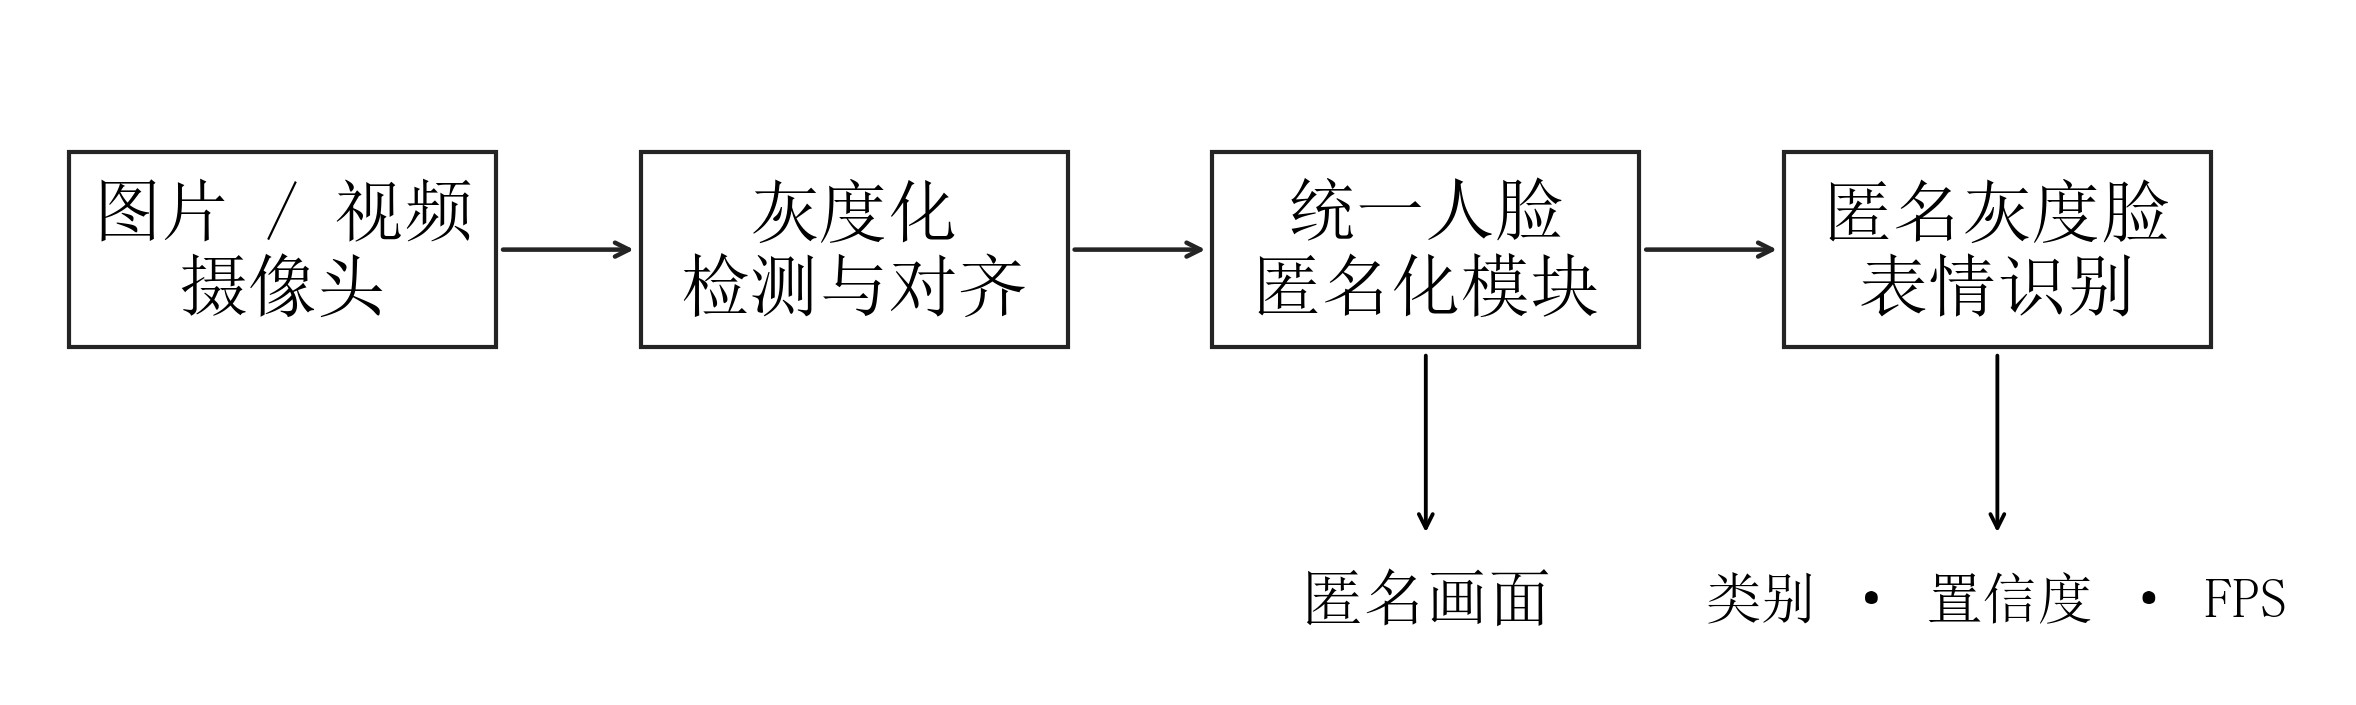
\includegraphics[width=\linewidth]{pipeline_diagram.png}
\caption{先匿名、后识别的系统处理流程}
\label{fig:pipeline}
\end{figure}

图\ref{fig:pipeline}中，原始画面只在采集、定位、匿名处理及对照显示中使用。表情调用位于匿名化之后；身份模型作为离线评价工具，用于比较同一输入在处理前后的身份预测变化，不参与视频中的表情判断。

\subsection{模块输入与输出}
检测模块使用 YuNet 定位人脸，并输出双眼、鼻尖和嘴角五点。对齐模块根据五点求取相似变换，减小尺度、平移和面内旋转的影响。统一坐标后，局部掩膜能够稳定覆盖面部，匿名结果也能合成回原画面的相应位置。

\begin{table}[htbp]
\centering
\caption{系统模块及其输入输出}
\label{tab:io}
\begin{tabularx}{\linewidth}{@{}lXX@{}}
\toprule
模块 & 输入 & 输出\\
\midrule
采集与灰度化 & 图片或视频帧 & 单通道灰度画面\\
人脸检测与对齐 & 灰度画面 & 人脸框、五点与对齐脸\\
统一匿名化 & 对齐人脸、区域约束 & 匿名画面与匿名灰度脸\\
表情识别 & 匿名灰度脸 & 七类概率与当前类别\\
时序决策 & 当前及历史匿名帧概率 & 稳定类别、置信度与状态\\
桌面展示 & 图像、分析结果与计时信息 & 对照画面与结果面板\\
\bottomrule
\end{tabularx}
\end{table}

\subsection{匿名化输入边界}
系统将分类输入定义为从实际匿名结果重新对齐得到的 $100\times100$ 灰度人脸。处理顺序为
\begin{equation}
 I_{\mathrm{raw}}\longrightarrow I_{\mathrm{gray}}
 \longrightarrow I_{\mathrm{anon}}\longrightarrow x_{\mathrm{expr}}.
\label{eq:chain}
\end{equation}
其中 $x_{\mathrm{expr}}$ 不从原图直接裁取。运行接口记录 \texttt{anonymized\_only} 来源标记；质量分类接口还检查数据类型、尺寸、标签顺序与模型校验值，使输入条件落实到程序调用中。

训练同样遵守这一边界。匿名缓存先保存运行流程得到的灰度脸，再与真实表情标签配对。分类器学习匿名域中的表情结构，不需要先预测原图类别，也不利用相似表情图片覆盖输入。

\subsection{人脸匿名化模块}
局部残差组件采用单通道 U-Net。编码器提取多尺度特征，解码器结合跳跃连接恢复空间结构，输出经过双曲正切函数限幅后与输入相加：
\begin{equation}
 A(x)=\operatorname{clip}\!\left(x+0.25\tanh R_\theta(x),0,1\right).
\label{eq:residual}
\end{equation}
限幅残差使网络围绕原有亮度与姿态进行局部编辑。关键点条件组件根据几何线图生成面部内容；生成器读取条件图，原始脸部像素不直接作为生成器输入。

合成时，软掩膜 $M$ 将编辑范围限制在面部内部，输出为 $I_{\mathrm{out}}=M\odot I_{\mathrm{edit}}+(1-M)\odot I_{\mathrm{gray}}$。掩膜外保留灰度输入像素，边缘采用渐变过渡，使面部修改与头发、背景自然衔接。

匿名化训练联合使用像素重建、匿名图表情标签、身份特征抑制与总变分平滑约束。身份项依据自建模型的面部特征与分类输出构造，推动匿名结果降低原身份关联；表情项使用匿名输出和真实标签，使身份编辑与表情保留在同一训练目标中协调。

\subsection{表情识别与桌面端}
实时表情网络使用四组卷积块，通道数依次为 32、64、128、192，经池化和投影得到 128 维特征，再输出七类表情。质量配置使用固定版本的 ENet-B2 表征\cite{emotieff}，将匿名输入缩放为 $260\times260$，扩展三通道并归一化；结合翻转测试时增强与温度校准输出概率。

视频中，因果时序滤波器累计连续帧的证据，减小孤立预测引起的跳变。轨迹重建、失脸或证据不足时更新识别状态。PySide6 桌面端通过工作线程执行推理，PyAV 负责视频编解码；页面负责显示结果，避免模型计算阻塞界面操作。
